As previously mentioned, radial distortion is only dependent on the distance between the origin and the point being considered.
Because of this, it can be thought of as a transformation which, according to some function $f$, moves the point to a different location on the line intersecting it and the origin.
More specifically, for a point $(r_u, \theta_u)$ in polar coordinates, $r_d = f(r_u), \theta_d = \theta_u$ is a radial distortion where $(r_d, \theta_d)$ represents the distorted polar coordinates of the point.

Brown's model for lens distortion~\cite{brown1966decentering} builds upon that presented by Conrady~\cite{conrady1919lens}, presenting a mathematical representation of barrel/pincushion and tangential distortion.
The rest of this report will consider a simplified version of this model in which there is no tangential distortion and is evaluated up to $r^5$ (and $r^8$ for its inverse).
This simplified version of Brown's radial distortion model is shown in Eq.~\ref{eq:brown-forward-radial-distortion}.
The approximation of its inverse is shown in Eq.~\ref{eq:brown-inverse-radial-distortion}.

\begin{equation}
    \label{eq:brown-forward-radial-distortion}
    r_d = f(r_u) = r_u + c_1 r_u^3 + c_2 r_u^5
\end{equation}

\begin{equation}
    \label{eq:brown-inverse-radial-distortion}
    r_u = f^{-1}(r_d) \approx \frac{c_1 r_d^2 + c_2 r_d^4 + c_1^2 r_d^4 + c_2^2 r_d^8 + 2 c_1 c_2 r_d^6}{1 + 4 c_1 r_d^2 + 6 c_2 r_d^4}
\end{equation}

Where $c_1$ and $c_2$ are per-lens constants that determine the extremity of the distortion.
These are usually calculated experimentally, however, for the static renders in this paper, they will be set to arbitrary values of $c_1 = 0.15$ and $c_2 = 0.10$.
While these are relatively extreme, they clearly exemplify the concepts being demonstrated.
Its worth noting that, due to the approximate nature of the inverse distortion function, the greater values of $c_1$ and $c_2$, the more $f^{-1}(f(r))$, $f(f^{-1}(r))$ and $r$ diverge.

For practical implementations, computers represent points using cartesian coordinates.
Because of this, any transformations first need to convert the coordinates to polar form.
Given a two dimensional cartesian point $p = (x, y)$, its polar form is $\left(r = \sqrt{x^2 + y^2} = \sqrt{p \cdot p}, \theta = \arctantwo{(y, x)}\right)$.
Given a two dimensional polar point $(r, \theta)$, its cartesian form is $\left(x = r \cos{\theta}, y = r \sin{\theta}\right)$.

By using the fact that only $r$ is varied during a radial distortion, an optimisation can be used whereby only $r$, or the required powers of $r$, are calculated, and the cartesian coordinates are simply scaled by that applied during the distortion (removing the need to calculate $\theta$, $\sin{\theta}$, and $\cos{\theta}$).
Applying this to Brown's model, for a point $(x_u, y_u)$,~\cite{mallon2004precise} calculates its distorted point $(x_d, y_d)$ as shown in Eq.~\ref{eq:inverse-radial-distortion}.

\begin{equation}
    \label{eq:inverse-radial-distortion}
    \binom{x_u}{y_u} = \binom{x_d}{y_d} \left(1 - f^{-1}\left(\sqrt{x_d^2 + y_d^2}\right)\right),
\end{equation}

All distortions are applied on top of the scene shown in Fig.~\ref{fig:no-distortion}.
Any intermediary render textures are $1024 \times 1024$ pixels and the output resolution is $500 \times 500$ pixels unless otherwise specified.

\begin{figure}[ht]
    \centering
    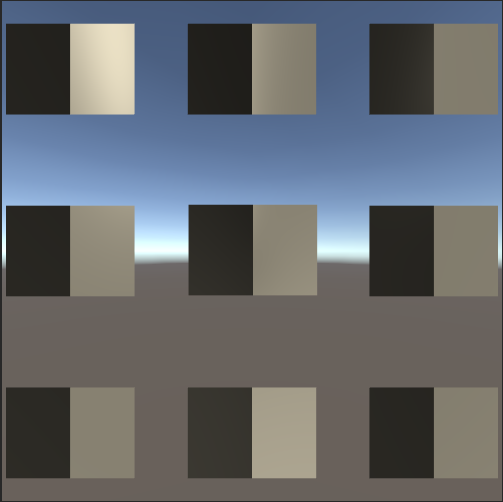
\includegraphics[width=0.4\textwidth]{figures/no-distortion}
    \caption{Untouched and undistorted 9-cube scene.}
    \label{fig:no-distortion}
\end{figure}

\subsection{Pixel-based Distortion Correction}\label{sec:pixel-based}

The pixel-based distortion correction method works by transforming UV positions in the texture map for each pixel (or fragment).
In a normal fragment shader, the graphics card provides texture UV positions (between $(0, 0)$ and $(1, 1)$) interpolated between those specified in the vertex shader.
A \texttt{sampler2D} is then used to retrieve the colour of the pixel in the texture corresponding to the UV position.
In order to perform distortion, the UV position being sampled can be changed.

Firstly, both the forward and inverse radial distortions functions require points to be normalised to between $(-1, -1)$ and $(1, 1)$.
For input UV position $p_{\texttt{UV}}$, this is achieved simply using $p_{\texttt{norm}} = 2 p_{\texttt{UV}} - 1$.
After the distortion transformation is completed, the normalised points are converted back to UV positions using $p_{\texttt{UV}}' = 0.5 (p_{\texttt{norm}}' + 1)$.

Somewhat non-trivially, to perform a radial barrel or pincushion distortion, the opposite equation must be used (Eq.~\ref{eq:brown-forward-radial-distortion} for barrel and Eq.~\ref{eq:brown-inverse-radial-distortion} for pincushion).
This is because sampling a different UV value to the current one is already the inverse operation.
Instead of imagining the current UV point $A$ being transformed to its distorted UV point $B$, its better to think of it as finding the UV point that should replace $A$, and calculating this to be $B$.
Hence, for barrel distortion, considering the point $A$, it needs to be replaced by a point $B$ further away from the origin (effectively distorting by compression).
In this case, $B$ is found by inverting the distortion that lands on $A$, therefore using Eq.~\ref{eq:brown-forward-radial-distortion} (and vice versa for pincushion distortion).

The fragment shader implementation simply performs this operation for each pixel/fragment in the image, and discards any fragments who's distorted UV positions lie outside the bounds of the texture.
The results of this and simulation of it running through a lens are shown in~\ref{fig:frag-based}.

\begin{figure}[ht]
    \centering

    \subfloat[Pre-distortion]{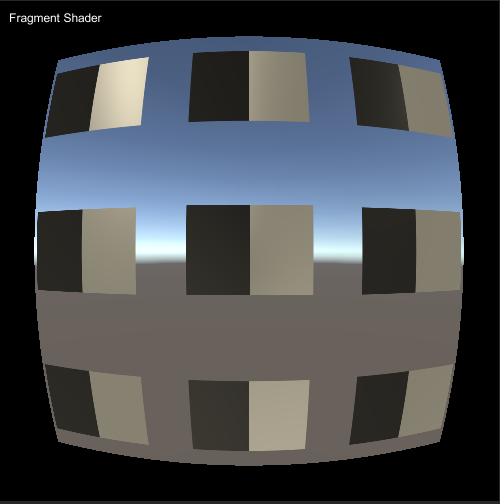
\includegraphics[width=0.225\textwidth]{figures/pixel-based}}
    \hfil
    \subfloat[Correction and distortion]{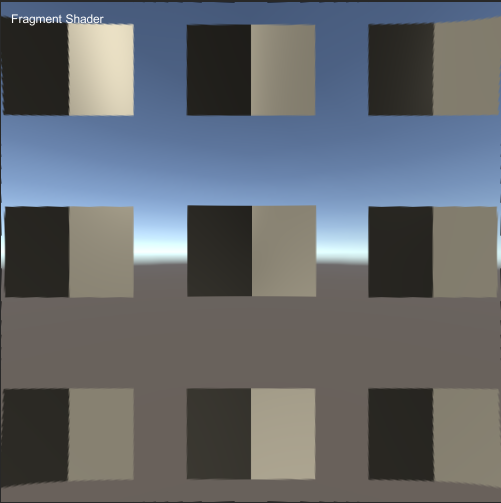
\includegraphics[width=0.225\textwidth]{figures/pixel-based-inverse}}
    
    \caption{Pixel-based pre-distortion and lens simulation.}
    \label{fig:frag-based}
\end{figure}

\subsection{Mesh-based Distortion Correction}\label{sec:mesh-based}

The mesh-based distortion correction method works by transforming the vertex positions of a mesh (instead of transforming texture UV positions).
In doing so, it looks to exploit the graphics rendering pipeline for a performance gain with minimal residual artifacts.

The meshes were produced in Blender by continually subdividing a plane (the $8 \times 8$ mesh is shown in Fig.~\ref{fig:blender-mesh8}).
An $n \times n$ mesh has $n^2$ quads, $2n^2$ triangles, or $(n + 1)^2 = n^2 + 2n + 1$ vertices.
As each face is subdivided into four subfaces, $n$ is a power of $2$.

\begin{figure}[ht]
    \centering
    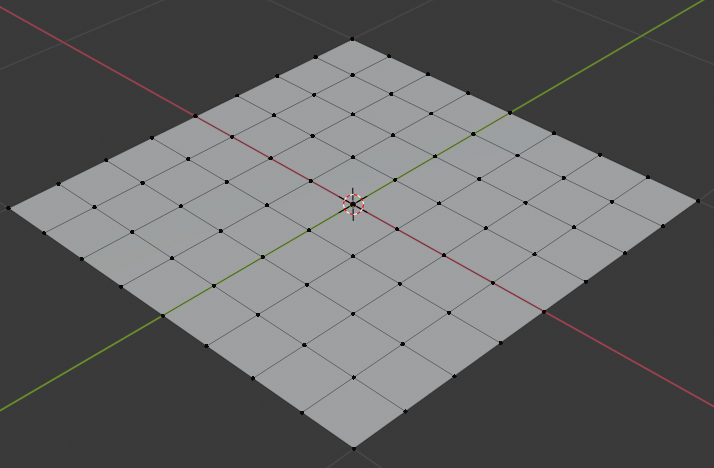
\includegraphics[width=0.4\textwidth]{figures/blender-mesh8}
    \caption{$8 \times 8$ mesh in Blender.}
    \label{fig:blender-mesh8}
\end{figure}

In the vertex shader, vertices are first transformed from world-space to clip-space using its model-view-projection matrix.
Since clip-space is between $(-1, -1)$ and $(1, 1)$, it matches the domain of both Eq.~\ref{eq:brown-forward-radial-distortion} and Eq.~\ref{eq:brown-inverse-radial-distortion}.
This means that the respective radial transforms can be applied to the vertices in clip-space to distort their positions.

Opposite to the pixel-based method, applying pre-distortion correction to the output requires the inverse radial transform (Eq.~\ref{eq:brown-inverse-radial-distortion}), and simulating the distortion requires the forward radial transform (Eq.~\ref{eq:brown-forward-radial-distortion}).
This works by translating the vertices (as if they were distorted) to their pre-distorted positions.
As part of the rendering pipeline, during the fragment shader, each of these pre-distorted vertex positions are linearly interpolated by the graphics card to produce estimates for pre-distorted fragments/pixels.

In order to simulate a lens being applied to the pre-distorted image, as mentioned, the same technique is applied using the forward radial transform (Eq.~\ref{eq:brown-forward-radial-distortion}).
This then cancels out the pre-distortion to produce an image similar to that which was input ($f^{-1}(f(r)) = r$).

As an aside, similar results could be achieved by performing the same texture UV transformation in the vertex shader as that used by the pixel-based method in the fragment shader.
While this would cause the same distortion, as vertices remain on the edge, a mesh image of original size would be output, causing redundant additional distortion and calculations near the edge (instead of the black background).

Fig.~\ref{fig:mesh-based-distortion} shows the mesh-based method applied to three meshes ($8 \times 8$, $128 \times 128$, and $512 \times 512$) with correction only ($a$, $c$, and $e$) and correction with distortion ($b$, $d$, and $f$).
The main visible difference is between $8 \times 8$ and $128 \times 128$, where clear straight lines blend into curved lines.
There is also a clear difference in correction and distortion applied together, with the $8 \times 8$ mesh exhibiting clear artifacts towards the corners.
Between $128 \times 128$ and $512 \times 512$ there is no perceivable difference in output, implying that at this level the difference is sub-pixel.
This makes logical sense since the number of quads (and by extension vertices) exceed the number of pixels in the image.

\begin{figure}[ht]
    \centering
    
    \subfloat[$8 \times 8$ mesh, corrected]{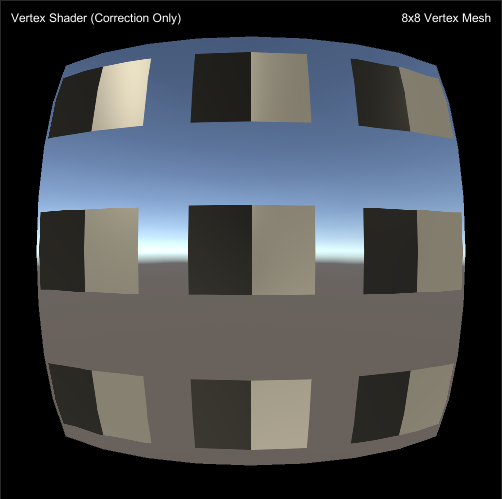
\includegraphics[width=0.225\textwidth]{figures/mesh-based-correction8}}
    \hfil
    \subfloat[$8 \times 8$ mesh, corrected and distorted]{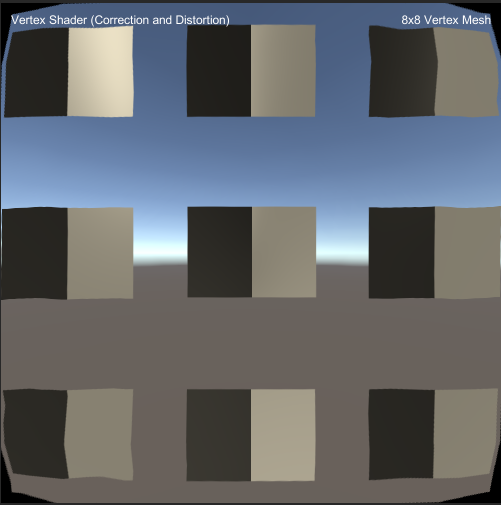
\includegraphics[width=0.225\textwidth]{figures/mesh-based-distortion8}}
    
    \subfloat[$128 \times 128$ mesh, corrected]{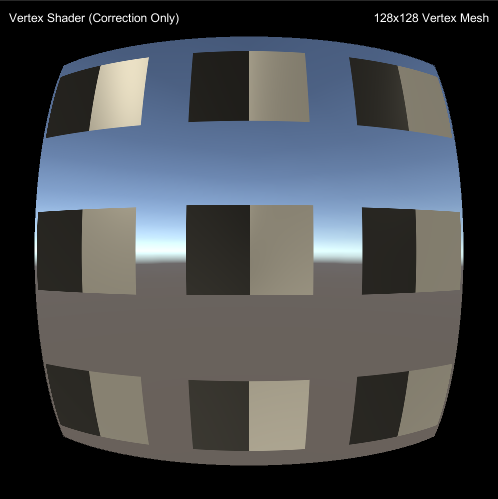
\includegraphics[width=0.225\textwidth]{figures/mesh-based-correction128}}
    \hfil
    \subfloat[$128 \times 128$ mesh, corrected and distorted]{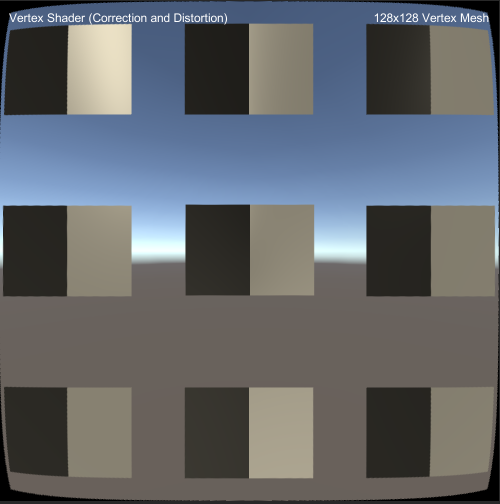
\includegraphics[width=0.225\textwidth]{figures/mesh-based-distortion128}}
    
    \subfloat[$512 \times 512$ mesh, corrected]{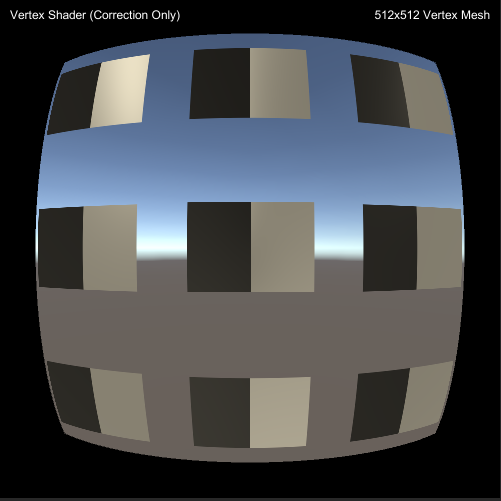
\includegraphics[width=0.225\textwidth]{figures/mesh-based-correction512}}
    \hfil
    \subfloat[$512 \times 512$ mesh, corrected and distorted]{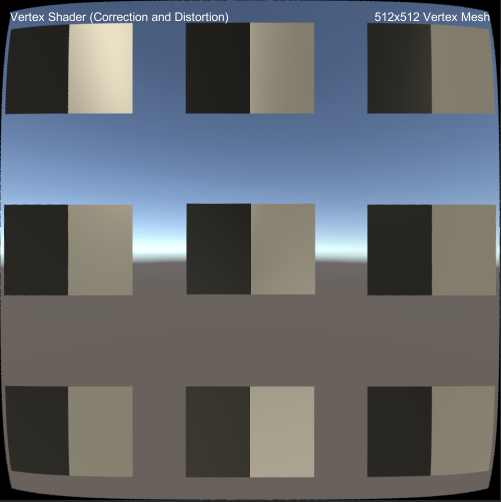
\includegraphics[width=0.225\textwidth]{figures/mesh-based-distortion512}}
    
    \caption{LCA pre-distortion and corrected LCA with distortion.}
    \label{fig:mesh-based-distortion}
\end{figure}

For benchmarking and profiling, on an i7 6700K with an RTX 2080 at $500 \times 500$ pixels, all three meshes performed the same (about 1.7ms per frame).
However, increasing the resolution to $8192 \times 8192$ yields more reliable variation on the frame rate and a clear performance drop as mesh complexity increases.
The profiling results are shown in Tab.~\ref{tab:benchmarking}.
These results, combined with the minimal visual difference between the more detailed meshes, show that a low-poly mesh is a good trade-off between frame rate and visual quality.

\begin{table}[ht]
    \centering
    \caption{Profiling results for three meshes at $8192 \times 8192$ resolution.}
    \label{tab:benchmarking}
    \begin{tabular}{c|cccc}
    \textbf{Mesh}     & \textbf{FPS} & \textbf{CPU (ms)} & \textbf{GPU (ms)} & \textbf{Total (ms)} \\ \hline
    $8 \times 8$      & $\sim135$    & $7.3$             & $0.3$           & $7.3$                 \\
    $128 \times 128$  & $\sim128$    & $7.8$             & $0.3$           & $7.9$                 \\
    $512 \times 512$  & $\sim104$    & $9.4$             & $0.3$           & $9.5$                
    \end{tabular}
\end{table}

\subsection{Pixel-based vs Mesh-based Distortion Correction}\label{sec:pixel-vs-mesh-based}

Both techniques have advantages and drawbacks.

Firstly, pixel-based pre-distortion in the fragment shader involves calculating Eq.~\ref{eq:brown-forward-radial-distortion} for each fragment/pixel in the scene, including those which are eventually discarded.
On the other hand, mesh-based pre-distortion in the vertex shader involves calculating Eq.~\ref{eq:brown-inverse-radial-distortion} for each vertex in the mesh.
This means that, for a mesh with far less vertices than pixels being rendered to the screen, the mesh-based method performs far less direct distortion calculations than the pixel-based method, giving it better theoretical performance.

Secondly, while the pixel-based method produces the most accurate theoretical discrete output, in practice, the mesh-based method is able to produce indistinguishable results for a low number of vertices relative to pixels/fragments.

From an implementation efficiency standpoint, one drawback of the mesh-based method is that using Eq.\ref{eq:brown-inverse-radial-distortion} means it needs to perform more operations per vertex calculation than the pixel-based method does per pixel.
It does however have the added benefit that the input coordinates are already normalised to between $-1$ and $1$.
Additionally, since it only uses even powers of $r$, $r^2$ can be trivially calculated using $r^2 = x^2 + y^2 = p \cdot p$, removing the need for an expensive square root.

For the frame buffer resolution of $1024 \times 1024$ pixels used in the render targets, the fragment shader in the pixel-based method should perform $1024^2 = 1048576$ distortion calculations and up to $1048576$ texture lookups per frame (dependent on the number of discarded fragments).
On the other hand, the mesh-based method only performs $(n + 1)^2$ distortion calculations for an $n \times n$-quad mesh ($81$ calculations for $8 \times 8$, $16384$ for $128 \times 128$, and $262144$ for $512 \times 512$), but will still require up to $1048576$ texture lookups as the fragment shader samples the texture for each fragment in the buffer.

Finally, while not used in this report, the mesh-based method can be further refined by pre-baking its distorted vertex positions, removing the need to do any distortion calculations at runtime.
